\documentclass{article}
\usepackage{../assignment_preamble}

\title{Homework 1}
\author{Ravi Kini}
\date{October 1, 2025}

\begin{document}

\maketitle

\problem
\begin{center}
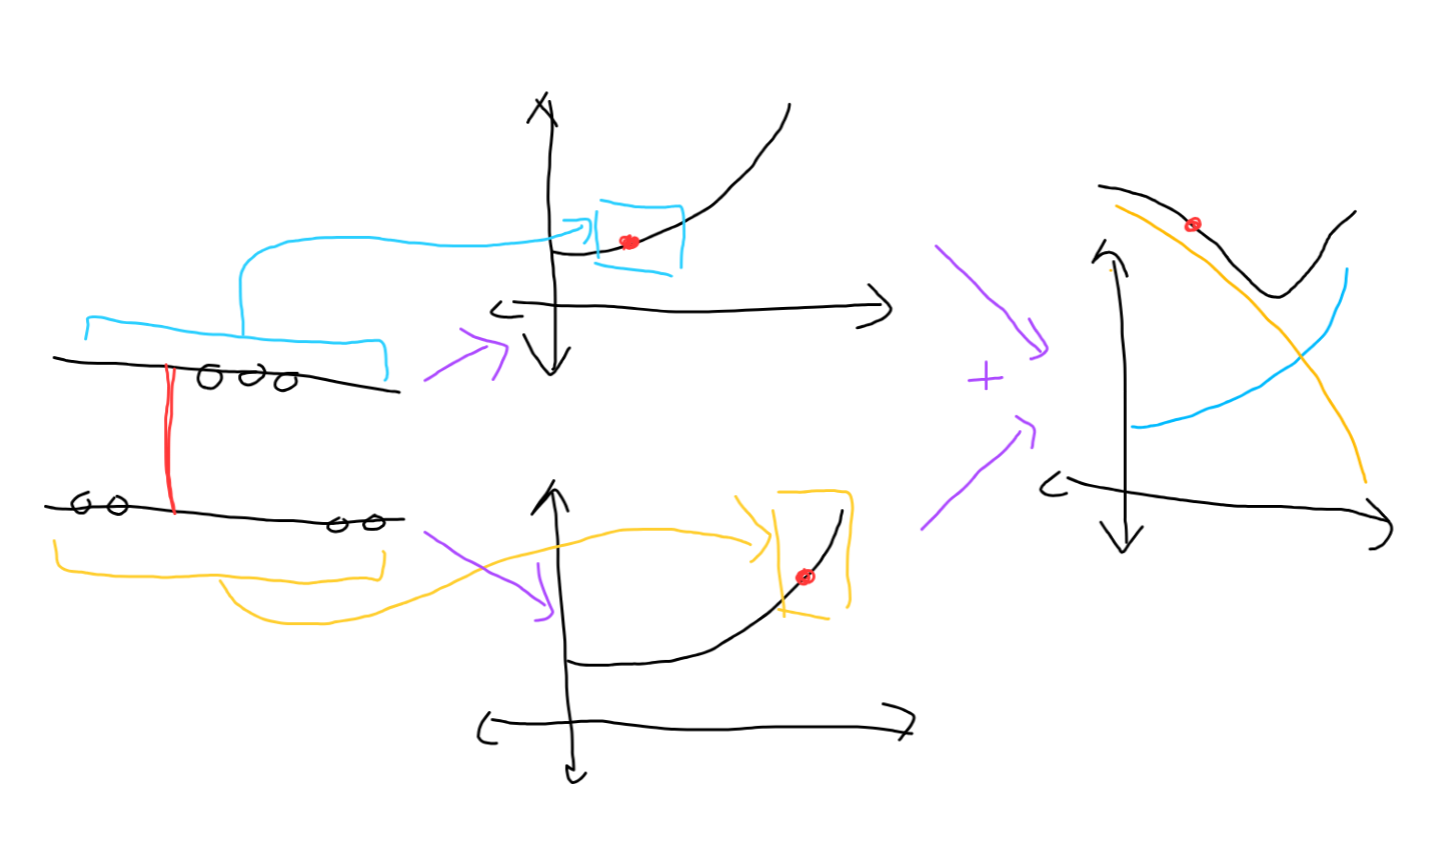
\includegraphics[width=0.6\textwidth]{../../img/inference_machine.png}
\end{center}
The inference machine works by linearly mapping the dosage to sections of the activation functions, then taking the weighted sum to get the efficacy. The dosage is first multiplied by a factor referred to as a weight, and then offset by the bias. These quantities are determined through a process called backpropagation. The result is then fed into a function referred to as an activation function; the inference machine in the video uses a softplus function. Finally, the outputs of the individual activation functions are multiplied by another factor and then added to produce the efficacy.

\clearpage

\problem
Each atomic sentence can be either true or false. Since individual atomic sentences' truth values are independent, there are $2^n$ possibilities for the values of $n$ atomic sentences, and $2^n$ rows are required for the truth table.
\end{document}